% Evidence-based research priorities after the shared first-stage evaluation.
\documentclass[11pt,a4paper]{ctexart}
\usepackage[margin=2cm]{geometry}
\usepackage{amsmath,amssymb,booktabs,tabularx,graphicx,enumitem}
\usepackage[colorlinks=true,urlcolor=blue]{hyperref}
\setlist{nosep,leftmargin=2em}
\setlength{\parskip}{4pt}
\setlength{\parindent}{2em}
\newcommand{\sk}[1]{[#1]_\times}
\title{IMU--UWB 不变定位：下一步研究方向评估}
\author{Codex}
\date{2026年11月7日}
\begin{document}
\maketitle
\section{研究决策与证据}
建议集中推进\textbf{可观性与不确定度感知的冷启动及中断后再捕获，接单一InEKF跟踪器}；
将\textbf{间歇测距下偏置几何与可观性一致EqF}保留为理论备选。
这些是研究建议，尚未实现或证明，不同时铺开两条主线。

原论文Oursland与Mehrabian（RO-MAN2024）关注大初始航向误差的收敛，采用有杆臂TDoA。
本项目的平方距离提升旨在减少错误位置线性化的影响；目标应保持为扩大实际捕获域，
不预先认定某个提升形式必须胜出。当前零杆臂TWR不能与原论文数字直接排名。

本轮通过PowerShell/.NET逐样本重算126份NPZ、630条方法轨迹的主要位置指标、成功判定与有限性，
与CSV最大差为$1.4552\times10^{-11}$；12份源码指纹一致。
既有ESKF测试6项、捕获测试3项及不变模型/共同协议两组断言均通过。
没有重跑全部滤波实验或修改估计器。

\begin{center}\small
\begin{tabular}{lrrrr}
\toprule
方法&LOSO/24&留出/90&中断/12&留出RMSE中位(m)\\\midrule
InEKF-15&17&62&5&0.3939\\
ESKF-15&20&76&3&0.3711\\
固定捕获初始化&20&75&8&0.3314\\
捕获初始化＋中断重置&20&75&10&0.3314\\
完整deep&19&61&2&0.3751\\\bottomrule
\end{tabular}\end{center}
成功要求终段持续$\le0.5$ m且观察不少于5 s。
deep中断末5 s误差中位9.235 m，简化重置0.151 m；二者没有共同成功对，不能比较配对成功恢复速度。
square中deep成功13/15、简化0/15，但简化阈内覆盖约97.7\%、末5 s约0.39 m，不能称其全面失效。
octagon/star中deep仅2/15、1/15，简化均15/15。

\section{先解释正常初值的早期峰值}
留出random在真值位置初始化时，捕获输出仍于0.02 s达到16.226 m误差；
InEKF/ESKF分别在0.00/0.01 s达到34.117/118.268 m。
源码前256次有效更新同时关闭硬拒绝和Huber降权。
这是核实的行为，但异常首批测距、宽先验、更新顺序和有限注入的因果贡献尚需消融。
\textbf{既要接受真实大初差，又不能把准确初值拉走}，是首选方向的具体切入点。

\clearpage
\section{与原论文及现有提升公式的对照}
原论文式(33)--(38)使用非线性距离差及不变误差变换；记标签位置为$p+R\ell$，则
\begin{equation}
h_{BA}(X)=\|p+R\ell-a_B\|-\|p+R\ell-a_A\|.
\end{equation}
当前TWR模型为$z_i=\|p-a_i\|+\beta_i+n_i$。
对零均值高斯$n_i$及方差$\sigma_i^2$，提升输出
\begin{align}
y_i&=\tfrac12[(z_i-\beta_i)^2-\sigma_i^2]-\tfrac12\|a_i\|^2
=q-a_i^\top p+\eta_i,\\
q&=\tfrac12p^\top p,\qquad
\operatorname{Var}(\eta_i)=d_i^2\sigma_i^2+\tfrac12\sigma_i^4.
\end{align}
常数观测行只对提升状态成立；完整有偏惯导不因此成为已证明全局收敛的线性系统。
若每次用局部$J_f=\partial f/\partial x$重建辅助态协方差，则
\begin{equation}
P_{xs}=P_{xx}J_f^\top,\quad P_{ss}=J_fP_{xx}J_f^\top,
\quad H_{\rm eff}=H_sJ_f.
\end{equation}
因此重建仍可能引入局部近似。CLIF现配置大初差失败不能推广为所有提升方法的数学证伪；
但也不足以继续无限调参。

\section{首选方向的数学落点：条件性捕获与交接}
正常阶段只运行一个15维tracker；启动或检测到失测/失配时建立短窗$\mathcal W$。
候选批量状态估计使用原始距离残差与IMU约束：
\begin{equation}
J=\|e_0\|_{P_0^{-1}}^2+\sum_k\|r_k^{\rm IMU}\|_{Q_k^{-1}}^2
+\sum_{(i,k)\in\mathcal W}\rho\!\left(
\frac{(z_{ik}-\beta_i-h_i(x_k))^2}{\sigma_i^2}\right).
\end{equation}
提升或WLS作为候选初始化手段，与鲁棒短窗原始距离优化竞争。
单标签零杆臂时$\partial h_i/\partial\psi=0$；yaw与偏置需要运动和时间关联，
不能因锚点数量足够就断言完整状态可观。

将目标变量记为$a$、其他变量记为$n$，从数据雅可比构建局部信息：
\begin{equation}
\Lambda=J_x^\top WJ_x,\qquad
\Lambda_{a\mid n}=\Lambda_{aa}-\Lambda_{an}\Lambda_{nn}^{\dagger}\Lambda_{na}.
\end{equation}
先按实际物理尺度归一化，再以QR/SVD识别可辨识子空间；
避免把强先验误当传感器新增信息。
\textbf{局部满秩不保证全局唯一解或真实误差上界}，仍需处理镜像/多极小值及新数据预测验证。
不能仅用低残差、小P或固定时长决定接管。

\clearpage
\section{交接必须解决的信息问题}
当前deep的输出混合$\hat p_o=(1-w)\hat p_C+w\hat p_T$原则上需要
\begin{equation}
P_o=(1-w)^2P_C+w^2P_T+w(1-w)(P_{CT}+P_{CT}^{\top}).
\end{equation}
共享IMU/UWB导致相关性；现在没有严格融合$P_o$。
首选路线研究短窗联合后验到单tracker的替换与传播，明确数据使用边界，
不把捕获使用过的测距再次当独立证据。
鲁棒代价的逆Hessian也不自动等于一致的后验协方差，需Monte Carlo覆盖率检查。

\begin{center}\small
\begin{tabularx}{\linewidth}{lX}
\toprule
论文应有的增量&应检验的内容\\\midrule
条件性捕获判据&哪些状态/方向当前可初始化；不可辨识时延迟或部分交接\\
不确定度交接&保留必要相关性，不虚假压缩未观方向，不重复计数\\
可靠性实证&减少准确初值峰值、错误接管和恢复失败，报告不可用时间\\
强简单对照&鲁棒WLS初始化、短窗IMU＋原始距离优化、固定捕获/重置\\\bottomrule
\end{tabularx}\end{center}
先争取条件性局部稳定、误差有界或可辨识结论；不预设完整有偏系统AGAS/GES。
若只是增加几条监督阈值或普通两秒优化重置，创新仍然不足。

\section{理论备选：偏置几何与间歇测距一致性}
原论文在$SE_2(3)$之外附加欧氏偏置，偏置耦合使无偏置的严格log-linear结构不再自动成立。
可以研究适合原始测距的bias-aware EqF及其退化运动/中断下的信息结构，
但半直积偏置EqF和range-only EqF已有前作。
\begin{enumerate}
\item 先选TWR或TDoA一种，推导群作用、lift、完整含偏置误差与测距输出。
\item 已知锚点限制对称性；不能照搬未知锚点SLAM或VIO的固定不可观方向。
\item 证明或数值检验未观方向不被虚假压缩，并隔离传播、量测近似、先验与有限注入的收益。
\item 若只是给2025测距EqF加偏置，或收益来自更宽P/不同Q，不足以支撑较强新颖性。
\end{enumerate}
当前共同不变核使用$F_r=C(X^+)F_eC(X)^{-1}$保证同离散物理模型，
有限群注入仍区别于ESKF的加性平移。
ESKF在本轮胜出不等于不变思想失效；换群也不是自动解决办法。
该路线先做2--3周理论可行性，再决定是否投入约4--6个月研究。

\clearpage
\section{已有工作对新颖性的约束}
\begin{itemize}
\item Goudar等，2024测距轨迹初始化：已有静态/恒速SDP松弛，多标签假设需区别。\newline
\url{https://arxiv.org/abs/2309.09011}
\item Ge等，ICRA2025测距EqF：已有无锚点方位初值的IMU＋range方法；未建模IMU偏置，实验说明使用合成测距补足缺口。\newline
\url{https://arxiv.org/abs/2503.03973}
\item Fornasier等，2025版：已有偏置半直积结构及瞬态比较。\newline
\url{https://arxiv.org/abs/2309.03765}
\item Ge等，CEP2026：正确重置条件下左右InEKF等价，不能包装左右切换/重置修正为新理论。\newline
\url{https://doi.org/10.1016/j.conengprac.2025.106656}
\item Liu与Shen，2026修订：线性观测群系统已有无偏置全局与强条件下有偏置半全局性质，需逐项核对适用条件。\newline
\url{https://arxiv.org/abs/2507.18493}
\item 本地eq\_ob教程是2026年3月v1；10月v3仍明确讨论相关AGAS构造同时估计偏置的困难。\newline
\url{https://arxiv.org/abs/2603.07143}
\item 时空标定与延迟几何已有2021 UWB--IMU和2026 Galilean EqF前作；当前0.20 s是共同传感器对真值的校正。\newline
\url{https://arxiv.org/abs/2108.00133}\quad
\url{https://arxiv.org/abs/2605.13266}
\end{itemize}
以上为针对性筛查，不宣称穷尽或首次性已证明。

\section{两周内先决定值不值得继续}
\begin{enumerate}
\item 记录random前0.1 s逐事件测距、创新、P、注入，拆解峰值来源。
\item 加入鲁棒WLS与短窗优化强基线，旧12条日志全部视为开发数据。
\item 用真实测距间隔因果触发恢复，去掉实验预先知道25 s的重启便利。
\item 预登记比较与失败规则，冻结参数，安排新日期/几何盲测。
\end{enumerate}
可暂以相对最强简单基线失败率下降30\%、正常p95恶化不超过5\%作为继续投入门槛；
这只是拟议工程取舍，不是已达结果或统计显著性标准。
若普通短窗优化已解决问题而新判据没有额外价值，应停止该新算法叙事。

\clearpage
\section{论文证据与会议计划}
当前初始化使用真值位置加偏移，不是真冷启动；12条TWR同日，全部有历史开发暴露。
90个扰动不能当90次独立采集。新方法必须在真实输入与真实可用先验下初始化，
按日志聚类给区间，并补新日期/几何或独立真实数据源。
有完整真值的仿真用于姿态/偏置误差和完整NEES；真实数据不捏造这些真值。
门控后NIS分布受选择影响，不能直接按未筛选卡方分布判断一致性。
保留固定0.5 m/5 s主指标，阈值敏感性只作辅助；报告所有未初始化、越界及观察不足。

\begin{center}\small
\begin{tabularx}{\linewidth}{lX}
\toprule
阶段&建议交付\\\midrule
第1--2周&因果诊断、强简单基线、冻结协议与继续决策\\
第3--5周&捕获判据、联合协方差交接、理论边界与退化反例\\
第6--9周&Monte Carlo、独立真实盲测、失测与NLOS分开测试\\
第10--12/14周&计算预算、主图、英文稿、失败分析与复现包\\\bottomrule
\end{tabularx}\end{center}

IROS级目标需要清楚的方法增量和可靠实验证据；主题较窄时IPIN等专业会议更匹配。
这是研究匹配判断而非官方评级/录用承诺。
ICRA2027常规论文延期截止为2026-09-16，已过；
PLANS2027摘要截止2026-10-16也已过，2月终稿不是新投稿入口。
本轮未可靠确认IROS/IPIN2027常规投稿期限，以正式CFP为准。

\noindent\href{https://2027.ieee-icra.org/announcements/call-for-papers-submission-deadline-extended/}{ICRA2027官方延期公告}
\quad\href{https://www.ion.org/plans/call-for-abstracts.cfm}{PLANS2027官方征稿}

\section{可视证据与交付边界}
\begin{center}
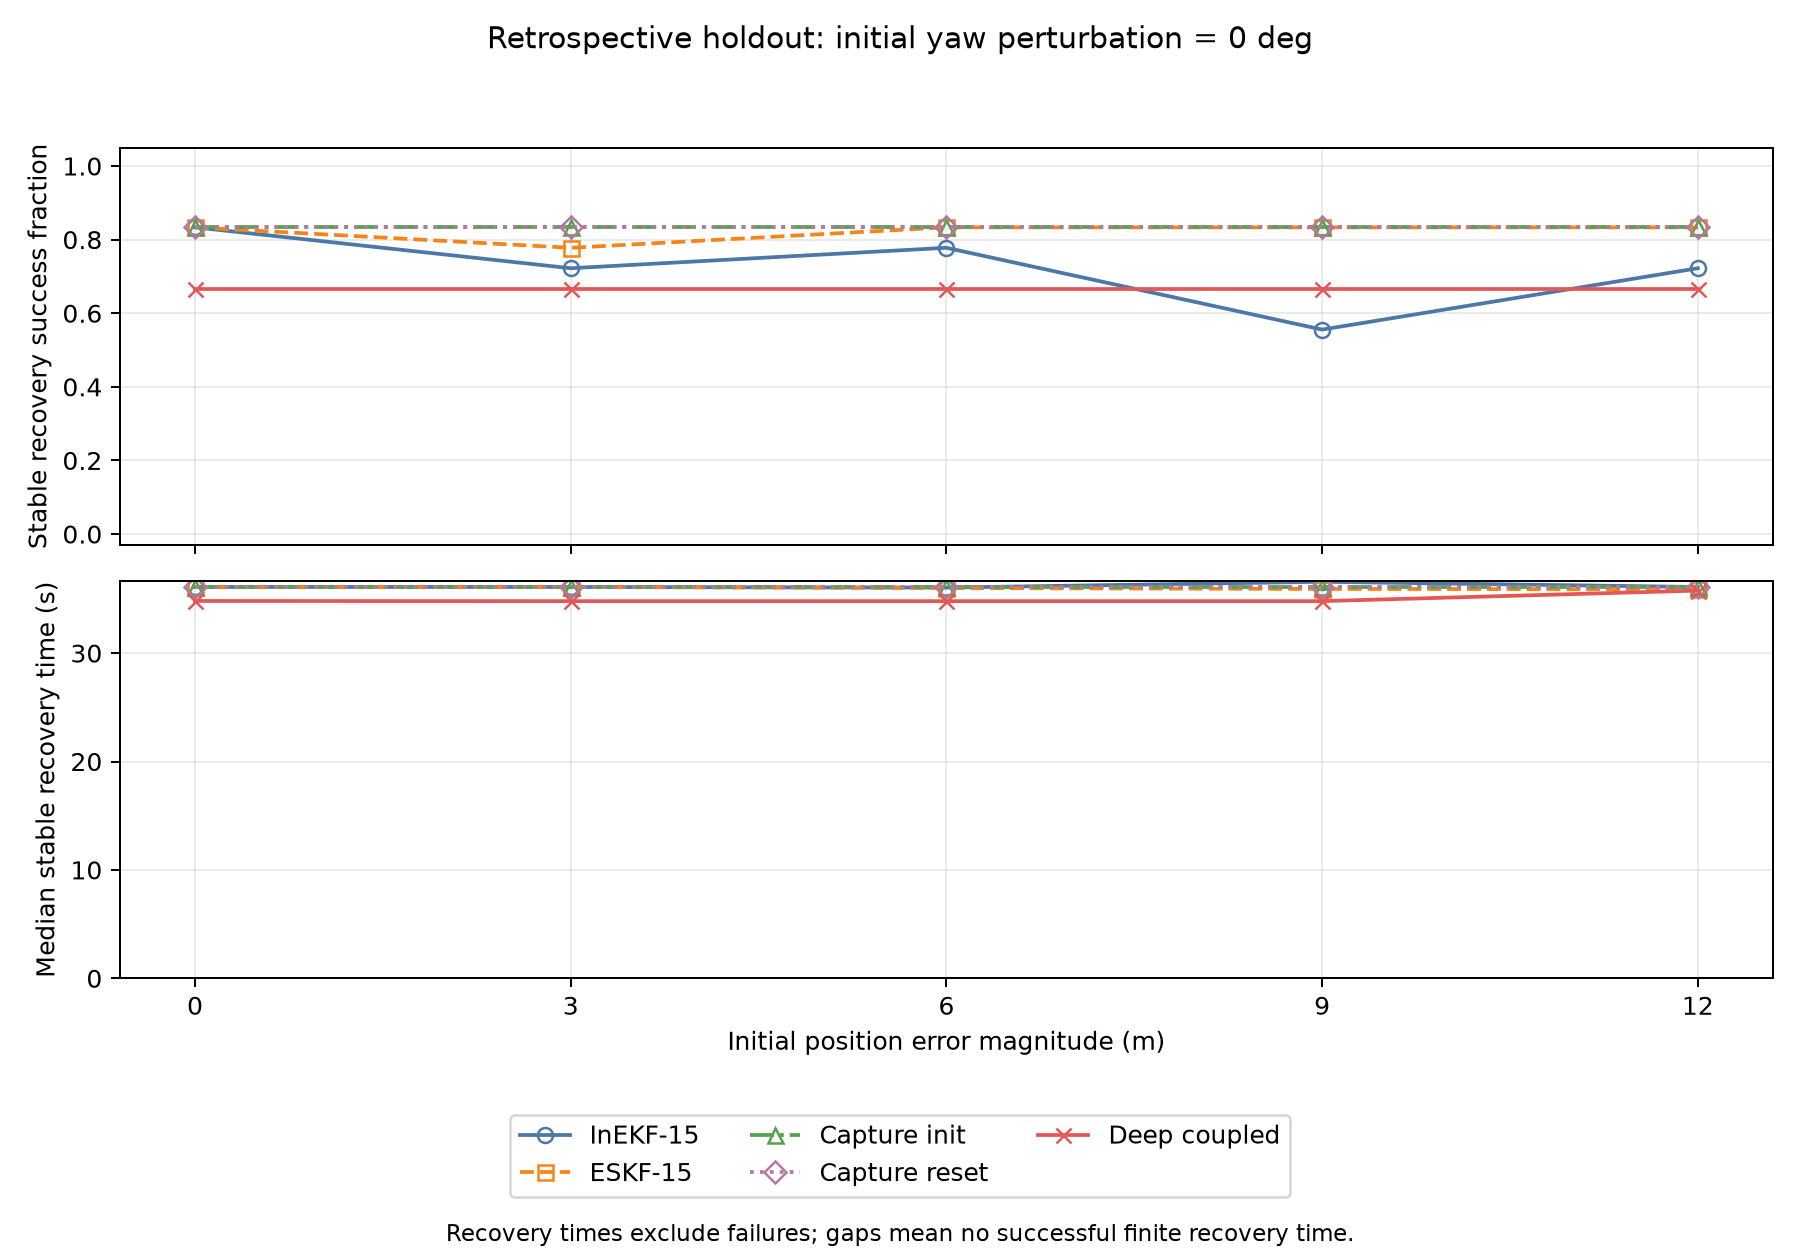
\includegraphics[width=0.72\linewidth]{../imu-uwb-inekf/results/roadmap_stage1_20261104_final/holdout_capture_domain.png}
\end{center}
图为\textbf{既有第一阶段结果}，不是本轮新方法结果。
本轮只新增研究评估和独立审计；没有实现新捕获算法、EqF、新盲测或收敛证明。
项目根.venv缺失，但原Conda环境可用，须配置其Library/bin运行路径；环境版本与冻结运行不完全相同。
完整决策、代码位置、复核限制和停止条件见同日\texttt{agent/report}报告。
\end{document}
